% This is mymiccaipaper.tex the demonstration file of
% MICCAI 2006 for Latex2e
% adapted from LLNCS.DEM from
% the LaTeX macro package from Springer-Verlag
% for Lecture Notes in Computer Science,
% version 2.2 for LaTeX2e
%
\documentclass{article}
\usepackage{fullpage}
%
\usepackage{makeidx}  % allows for indexgeneration
%

\usepackage[draft]{fixme}
\usepackage{color}
\newcommand{\mn}[1]{{\color{red}{#1}}}

\newcommand{\figheight}[1]{55mm}
\newcommand{\figwidth}[1]{0.45\linewidth}
\newcommand{\figfullwidth}[1]{0.9\linewidth}

\usepackage{graphicx}
\graphicspath{{pics/}{figs/}}
% list here all the paths to your figure folders
% \date{}


\begin{document}
%
%\frontmatter          % for the preliminaries
%
%\pagestyle{headings}  % switches on printing of running heads
%\pagestyle{empty}  % switches off printing of running heads
%
%\mainmatter              % start of your contributions
%
\title{Dynamic data analysis for pediatric airways}
%
%\titlerunning{Short Title}  % abbreviated title (for running head)
%
\author{Chun-Wei Liu}
%
%\authorrunning{C.-W. Liu}   % abbreviated author list (for running head)
%
%%%% modified list of authors for the TOC (add the affiliations)
%\tocauthor{Chun-Wei Liu (University of North Carolina at Chapel Hill)}
%
% \institute{Department of Computer Science,
% University of North Carolina, Chapel Hill, \email{chunwei@cs.unc.edu}
% }

% The following lines are used to remove authors and affiliations from
% the front page and running titles
%\author{Chun-Wei Liu}
%\authorrunning{C.-W. Liu}
%\tocauthor{Chun-Wei Liu (UNC-CH)}
%\institute{Department of Computer Science,\\
%University of North Carolina, Chapel Hill, NC\\
%\email{chunwei@cs.unc.edu}}

\maketitle              % typeset the title of the contribution

\begin{abstract}
The analysis of pediatric airway geometry using computed tomography (CT) images has provided rich diagnostic cues for doctors. Recently, dynamic CT data has started to provide a better characterization of pediatric airways throughout the breathing cycle, for example to assess tracheomalacia. However, how to preprocess the increasing amount of dynamic data and how to analyze these data are still open questions. In this work, I performed dynamic data analysis using computer vision and machine learning approaches on synthetic and real airway data. In the future, I aim at building a 4D atlas for pediatric airways and at extending the approaches to other dynamic data modalities.
\end{abstract}

\section{Introduction}
\label{sec:intro}
% Why this problem is important?

% What 3D CT can do?
The analysis of pediatric airway geometry using 3D computed tomography (CT) images has provided rich cues for doctors to diagnose respiratory issue for patients.
Both radiologists and physicians have been working on the field for a while.
In image analysis side, radiologists Nakanoa et al. started to propose algorithm for measuring airway lumenal area using multidetector row CT~\cite{nakano2002development} one decade ago.
On the other hand, physicians continuously adopted benefits from imaging analysis for their clinical studies, for example, how well their patients with issues caused by airway were recovered after surgeries~\cite{abramson2011three}.
The progress made in image analysis these days was making the communication of both parties much easier by providing more informative statics from images.
For instance, given a CT image from a subject with some manually annotative landmarks, machine is able to learn from CT images of normal control data to build a subject-specific control atlas (a mean statics from the population of the subject.) 
Then machine can provide statics for where the positions have smaller cross-sectional area to doctors which makes diagnosing tracheal stenosis more actuary~\cite{hong2014statistical}.

% What 4D CT can do?
What can we learn from a four-dimensional CT (4D) image, an image set contains up to 16 3D CT images with respiratory motion induced image changes across the set that are not available on a single-component 3D CT image?
If an edge of 3D CT images, comparing with spirometry, is on answering {\it where} a respiratory issue might be caused in the airway.
Then, 4D CT images provide even more information about {\it when} the respiratory issue might be caused in a respiratory cycle.

Four-dimensional CT imaging was developed to provide an estimate of tumor motion for radiotherapy treatment planning~\cite{ford2003respiration}.
After then, a method for dynamic ventilation imaging of the full respiratory cycle from 4D CT images was developed~\cite{guerrero2006dynamic}.
Recently, 4D CT imaging has started to provided a better characterization of pediatric airways throughout the breathing cycle, for example to assess tracheomalacia, which is a disease of temporally collapse of partial airway.

% Where are we now?
However, how to preprocess the increasing amount of dynamic data and how to analysis these data for pediatric airways are still open questions.
While standard techniques for analysis 3D CT images could be applied on analysis 4D CT images in a frame-by-frame fashion, two major challenges can be addressed as follow.
First, manual annotation labors or preprocessing costs of each subject has increased a factor proportional to the number of CT scans in a breath cycle.
Second, no information sharing between time steps makes temporal inconsistence for the analysis.
In this work, I am going to address the above issues by performing dynamic data analysis using computer vision and machine learning approaches.

% Where should we go?
In Section~\ref{sec:methods}, I will introduce the methods applying on pediatric airway analysis.
Experiments on real airway data would be compiled in on Section~\ref{sec:experiments}.
In Section~\ref{sec:discussion}, I will discuss about the future works, including building a 4D atlas for pediatric airways and extending the approaches to other dynamic data modalities.

\section{Methods}
\label{sec:methods}
\begin{figure}[tb]
  \begin{center}
    \begin{tabular}{ccc}
    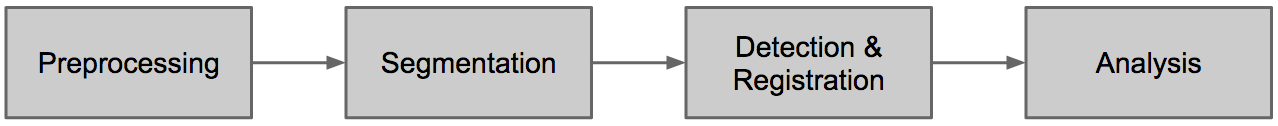
\includegraphics[width=\figfullwidth] {fig/framework.png}
    \end{tabular}
    \caption{ \label{fig:framework} Illustration of the proposed 4D CT image processing framework. From CT image preprocessing, image segmentation, landmark detection and functional data registration, to final analysis.
    }
  \end{center}
\end{figure}

% How do I approach it?
To perform data analysis for subjects with large spatial differences, spatial normalization in the form of registration is an important step.
Registration can be approached in different ways.
First, image registration, which uses image intensities as features, has been developed in medical image analysis for the past decade.
Most of these methods have to do with defining an energy function with data term (dissimilarity between source image and target image) and regularization term (atypicality of mapping from source image to target image),
and then develop optimization method to find a best mapping which minimizes such energy.
See the review articles by Hill et al. and Sotiras et al. on this topic~\cite{hill2001medical,otiras2013deformable} for details.
For particular application for registration on one subject among a short time period, Guerrero et al. developed a deformable algorithm for dynamic ventilation imaging from 4D CT~\cite{guerrero2006dynamic}.

On the other hand, shape registration, which uses geometric cues as major features, has succeeded in many applications in computer vision and computer graphics~\cite{belongie2002shape,li2012temporally}.
With the same fashion of energy minimization framework as image registration, these methods rely on shape features, e.g. curvature or level of bending, to define the data term.
However, using such techniques to align pediatric airway data is still difficult.
Hong et al. proposed a simplified airway model which allows for much easier registration for further analysis~\cite{hong2014statistical}.
In my work, I have the same interest of upper airway as Hong et al.
Figure~\ref{fig:Fleck} shows the anatomy I am looking at in this work.
I started this project by extending Hong et al.'s simplified airway model to a 4D CT processing framework.
Figure~\ref{fig:framework} illustrated the automatic 4D CT processing framework.


% Need to familiar with
\subsection{Image preprocessing and segmentation}
\label{sec:image_preprocessing_and_segmentation}
The algorithm segmented the airway from 3D CT image using Otsu's method and two manually chosen seeds that bracket the upper airway.
For better adaptive to current medical image processing libraries, the framework starts with transform data from DICOM images to NRRD images.
Then a padding and filtering operator for making the image boundary has the same intensity as air is applied on NRRD images.
With scripts automatically applying preprocessing programs reduced costs of manually operating medical image softwares, such as Slicer or ParaView.

Otsu's method finding a threshold to separate data into two clusters, so as to try to make each cluster as tight as possible.
This is achieved by maximizing the inter-subject variances and minimizing intra-subject variances in terms of voxel intensity.
In our case for segmenting airway, the two clusters were air and non-air regions.
To remove the air regions that were not in the airway, morphological operator erosion first be applied to remove the actual airway.
This computed a map of air regions outside the subject.
We can apply the map as a filter to remove the air outside the airway to get a clean airway in the subject.
Then, two seeds further help to extract trachea and exclude bronchus in the airway.

With this segmentation, the upper airway can be approximated by statical models~\cite{pizer2013nested}.
Focus on measuring the size of airway, we used a centerline with cross sections to represent the airway.
The centerline is inferred based on the heat distribution along the airway flow that is solved for by a Laplace equation.
Cross sections are cut from segmented airway geometry using planes that are orthogonal to the centerline. 
The area of the cross sections along the airway is then used as a 1D functional data representation of an airway.

\subsection{Landmark detection}
\label{sec:landmark_detection}
\begin{figure}[tb]
  \begin{center}
    \begin{tabular}{ccc}
    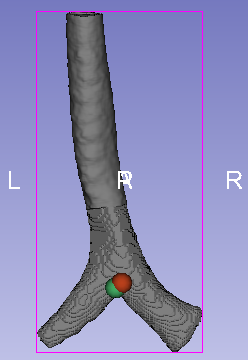
\includegraphics[height=\figheight] {fig/Fleck_005_geometry.png}
    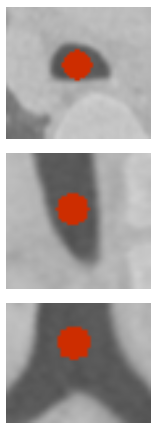
\includegraphics[height=\figheight] {fig/landmark.png}
    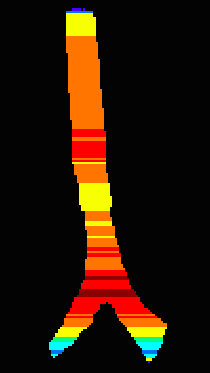
\includegraphics[height=\figheight] {fig/Fleck_005_likelihood.png}
    \end{tabular}
    \caption{ \label{fig:detection} Visualization of the framework of landmark detection. {\bf Left.} First, an airway geometry is segmented by Otsu-thresholding. Green marker is the ground truth annotation and red marker is the predicted location of TC. {\bf Middle.} Second, CHOG features are computed in the center of the trachea in each location along the airway. From top to down: Sagittal, coronal, and axial slices. {\bf Right.} Finally, results of applying the trained classifier on these different hypotheses to get likelihoods of the landmark. Dark red indicates the highest likelihood of TC. In this case, the predicted TC is only 1.97 mm (the total length of the airway is 159 mm) away from the ground truth annotation. This error is only 1.2$\%$ of the entire airway.
    }
  \end{center}
\end{figure}

We can register functional data using some common landmarks across subjects.
Typically landmarks are determined manually.
To reduce the manual annotation cost, based on Dalal and Triggs's object detection framework~\cite{dalal2005histograms}, I propose a landmark detection framework using concatenated Histogram of Gaussian (CHOG) features and a geometric prior. 
Figure~\ref{fig:detection} illustrates the detection of the trachea carina (TC).
The goal of the landmark detection is to capture the dynamics of landmarks.
Therefore, the accuracy of landmark detection should be higher enough to compensate the dynamics in the 4D CT image.
If the prediction error is larger than the actual dynamics in the 4D CT image, then the predicted location cannot be determined.

HOG is well designed normalized local histograms of image gradient orientation in a dense sample grid.
The original purpose of this feature was for human detection~\cite{dalal2005histograms}.
Given the popularity of HOG based object detectors, researchers even tried to answer why it works (or did not work) by visualizing the feature spaces~\cite{vondrick2013hoggles}.
However, it has more general applicability as it captures edge or gradient structures that are very characteristic of local shape. 
It can also be efficiently computed.
In practice the HOG is implemented by dividing an image window into small spatial cells, for each cell accumulating a histogram of gradient directions with different bins over pixels of the cell.
The concatenated histogram over cells would be the final representation of an image window. 
To apply HOG on 3D images, instead of computing histograms in arbitrary 3D orientations, I computed 2D HOG in the axial, coronal, and sagittal planes, which are the three perspectives for user annotations, and concatenated them together as a three times longer concatenated histogram (CHOG).
In this work, I used this simple trick to generalize HOG from 2D to 3D.

The first step of the landmark detection framework then is to train a binary classifier using CHOG.
For doing high dimensional data and low sample size statical analysis, Distance Weighted Discrimination can be applied to improve the training~\cite{marron2007distance}.
Yet, for simplistic and speed, linear Support Vector Machine (SVM) is used as a baseline throughout study.
In the prediction stage, the trained classifier can then be applied to the detect the particular landmark it was deigned for.
Higher score generally implies a higher likelihood of a hypothesis.

After landmarks are located, I registered the functional data using b-spline curve registration~\cite{ramsay2006functional}.
The technique needs at least four landmarks for registration.
In Hong et al.'s original paper, each subject had five visible landmarks: from nasal spine, choana, epiglottis tip, true vocal cord (TVC), and TC.
In our dynamic data, most of subjects only have TVC and TC due to a limited of view.
So we can only align these curves by fixing the start and the end of the curve and apply linear interpolation.
In some cases, TC is even the only available landmark which makes alignment impossible using linear interpolation.
I therefore apply a heuristic assumption to these special cases.
Given we have decent amount of data,
the assumption is that a given subject has the same length of trachea from TVC to TC as the most relevant subject (in terms of age) in our dataset.
Therefore, we can compute the proportion of the imaged trachea by measuring the ratio of the length of the current trachea in physical space and the length of the most relevant subject from TVC to TC.

\subsection{Statical atlas analysis}
\label{sec:statical_atlas_analysis}
Given spatially aligned functional data I would like to capture population changes with respect to some factors, say age.
We can use a blending kernel applying on the dataset to interpret a subject with the target age.
For example, I used a Gaussian weight function $w_i(a_i; \sigma, \bar{a}) = c\exp{(a_i-\bar{a})/2\sigma^2}$, where $a_i$ is the age for the observation $i$, $\sigma$ is a predefined standard deviation and $c$ is the normalization constant for fitting data to a specific age.

To further analyze the weighted data, I applied weighted functional boxplots to build a statistical atlas for each dynamic subject~\cite{hong2013weighted}.
Functional boxplots were originally proposed by Sun and Genton~\cite{sun2011functional} based on the definition of band depth for functional data.

Band depth is used to rank functional data for ordering it from the center outward.
To order functional data, we first define a subset and the membership of a data in the subset.
Given a functional dataset, any two function curves in the dataset can form a set in which the region between these two curves belong.
A curve is fully belong in this subset if it is in the region from the beginning to the end of the function.
A curve might be partially belong in the subset.
Figure~\ref{fig:vis_fbplot} shows the difference.
A band depth of a functional data curve can be defined as the ratio of the number of subset in which data is fully belong over all possible subsets.

\begin{figure}[tb]
  \begin{center}
    \begin{tabular}{ccc}
    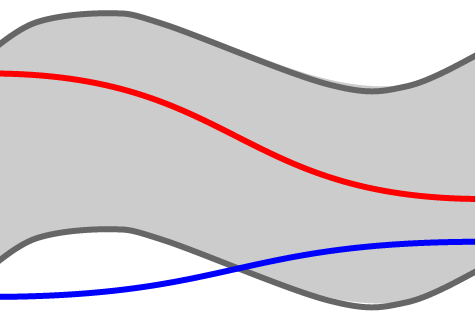
\includegraphics[height=35mm] {fig/illustration_fbplots.png}
    \end{tabular}
    \caption{ \label{fig:vis_fbplot} Visualization of the band depth. The red curve is fully belonged to the shaded region, but the blue curve is partially belonged to the shaded region.
    }
  \end{center}
\end{figure}

Given a set of functional data $Y=\{y_i | i=1,...,n\}$, a combinatorial function $C$ which enumerates all two pair combinations in a set, and a band function $B(y_1, y_2) = \{(t,x(t)): t\in \mathrm{T}, \mathrm{min}(y_1(t),y_2(t)) \leq x(t) \leq \mathrm{max}(y_1(t),y_2(t))\}$,
the band depth $D$ of a functional data $y$ with respect to a set $Y$ can be defined as

\begin{equation}
D(y; Y) = \sum_{y_i, y_j \in C(Y)} I[y \subset B(y_i, y_j)],
\label{eq:band_depth}
\end{equation}
where $I$ is an indicator function.
A generalize version of band depth is the weighted modified band depth

\begin{equation}
D'(y; Y) = \sum_{y_i, y_j \in C(Y)} w_iw_j\lambda[ B(y_i, y_j) ]
\label{eq:weighted_band_depth}
\end{equation}
where $\lambda$ is the Lebesgue measure, and $w$s are the weights of data for fitting the population.
If a curve $y$ is only partially in a subset $B(y_i,y_j)$, the $\lambda$ measures the ratio of time that $y$ is in the subset $B(y_i,y_j)$.
If a curve is fully in the subset, the $\lambda$ measurement is one.

When a rank of functional data is available, we can compute interesting statistics such as median, interquartile range, and outliers of the population.
I applied (\ref{eq:weighted_band_depth}) to compute a population atlas and to plot subject dynamics upon the population atlas using (\ref{eq:band_depth}).

\section{Experiments}
\label{sec:experiments}
% add data description
I applied the proposed framework on real world dynamic data.
This section will provide implementation details and parameter settings, and will also provide results and observations from experiments.

\subsection{Landmark detection results}
\label{sec:landmark_detection_results}
First I conducted a preliminary experiment before further developing landmark detection techniques by answering the question: How would landmark dynamics affect final airway analysis?

I studied this on the first dynamic data I got from our collaborator.
The subject was 59 days old and only had a TC annotation \footnote{The other annotation nearest TC was TVC, and it was not visible due to the doctor's choice of scan area}. 
I then chose the top of the airway as a dummy landmark TVC and the TC for registration.
I manually annotated the these two landmarks in each frame and computed the Euclidean difference between landmarks with respect to time.

Figure~\ref{fig:landmark_dynamics} shows the movement of landmarks between each frame in millimeter.
In this figure, TC shows a significant changes after time step 4.
The landmark dynamics revealed that the airway of the subject was changing a lot in a period of time.
%This observation matched our measurement of cross-sectional areas.

Figure~\ref{fig:landmark_updated} shows the results of the airway measurement of the 59 days old subject.
The difference between the left and right results in Figure~\ref{fig:landmark_updated} is whether considering the landmark dynamics.
The left result shows eight functional curves registered with the same TC and TVC annotation at the first frame.
The right result shows eight functional curves registered with the updated TC and TVC annotations at each frame.
We can see that Figure~\ref{fig:landmark_updated} (right) captured a cross-sectional area drop in the end of the functional data.
Figure~\ref{fig:landmark_updated} (left), however, lost this feature (compare the green curves on the left and on the right.)
Because an area drop is a critical feature for airway analysis, I considered updating landmarks in each time frame is an important issue and further developed the framework described in Section~\ref{sec:landmark_detection}.

\begin{figure}[tb]
  \begin{center}
    \begin{tabular}{ccc}
    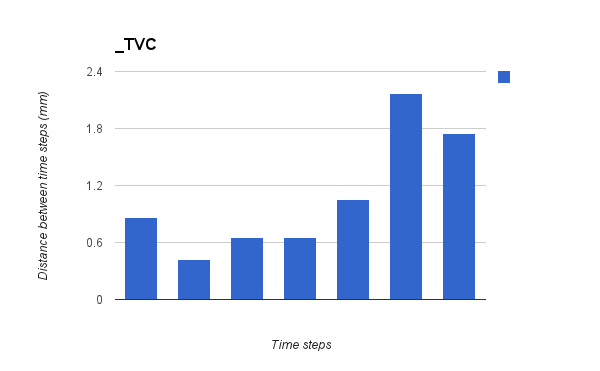
\includegraphics[width=\figwidth] {fig/d_TVC.png}
    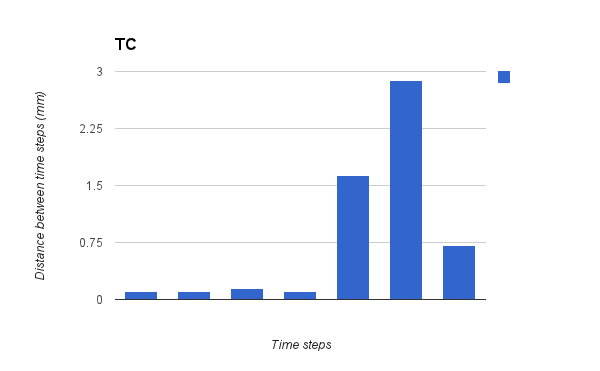
\includegraphics[width=\figwidth] {fig/dTC.png}
    \end{tabular}
    \caption{ \label{fig:landmark_dynamics} Visualization of the landmark dynamics of a 59 days subject. 
    }
  \end{center}
\end{figure}

\begin{figure}[tb]
  \begin{center}
    \begin{tabular}{ccc}
    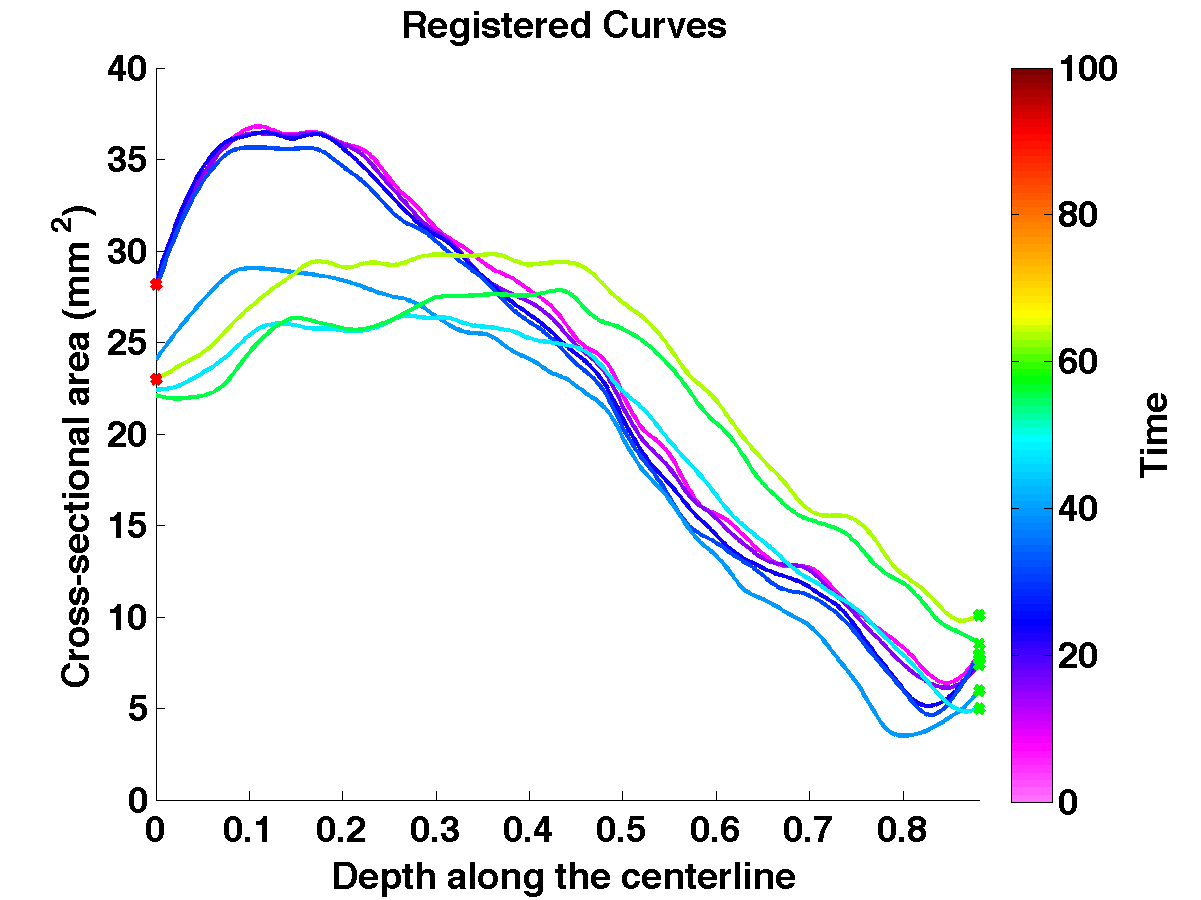
\includegraphics[width=\figwidth] {fig/registered_1_updates_0.png}
    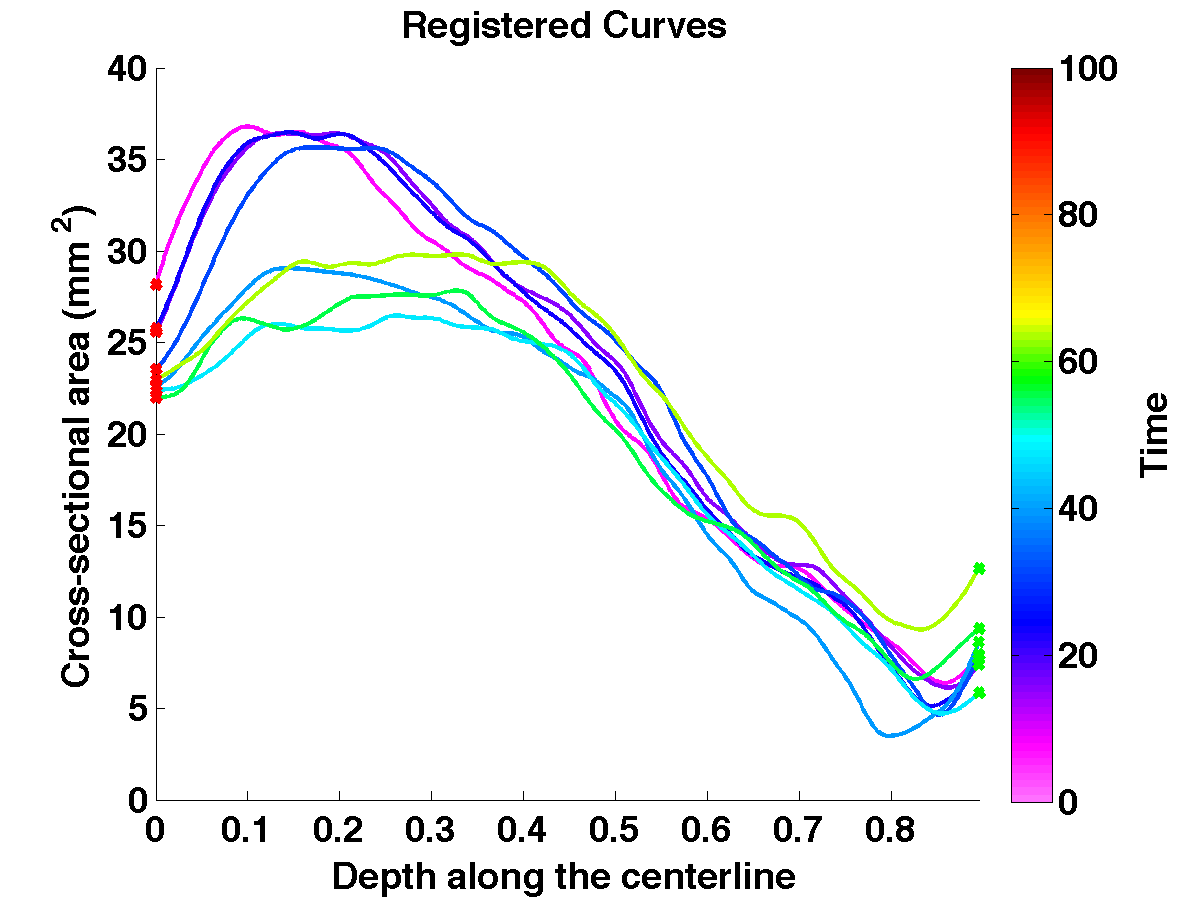
\includegraphics[width=\figwidth] {fig/registered_1_updates_1.png}
    \end{tabular}
    \caption{ \label{fig:landmark_updated} Cross-sectional area of a 59 days old subject with different registration landmarks. {\bf Left.} The result using the same landmarks for each time step. {\bf Right.} The result with updated landmarks for each time step. Note that in the end of functional data, a lower cross-sectional measurement disappeared on the left but remains on the right.
    }
  \end{center}
\end{figure}

Since updating landmarks with the subject's deformation is need, I applied the automatically landmark detector described in Section~\ref{sec:methods}.
The detector has training stage and detection stage.

{\bf Training.} 
The training set had 95 3D CT images with manually annotated landmarks from nasal spine, choana, epiglottis tip, TVC, and TC.
I trained a linear SVM classifier for TC using CHOG features.
Each subject provided a positive example which would be HOG features extracted from three orthogonal bounding boxes passing through the landmark TC.
The scale of the bounding boxes was chosen as twice of the minimum rectangle covering the airway in the axial plane.
The negative examples were drawn at an uniform distributed scale and location that did not intersect with the positive bounding boxes.
For each positive example, I drawn ten times negative samples.

{\bf Detection.}
For a 512$\times$512$\times$640 3D CT image, there are too many possible hypotheses of scale and location.
I utilized a prior of geometry to eliminate possible hypotheses.
Once we have the segmentation of the image, we only look at the segmented trachea for landmarks.
In each depth I only drew one hypothesis from the center of the airway using the scale with the same heuristic in training.
The trained SVM classifier predicted a score of the landmark likelihood given different depth.
Figure~\ref{fig:landmark_detection} illustrated the likelihood prediction on training data.
We can see there are some outliers in prediction on the training data.
Due to these outliers, the mean prediction error was 24.7436 (mm) and the standard deviation was 29.4251 (mm).

\begin{figure}[tb]
  \begin{center}
    \begin{tabular}{ccc}
    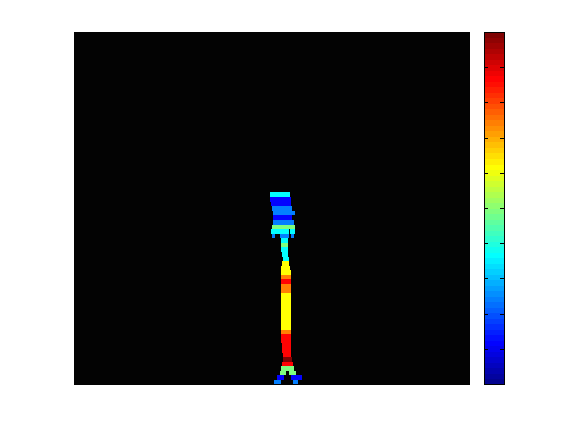
\includegraphics[width=\figwidth] {fig/CRL02_TracheaCarina_left.png}
    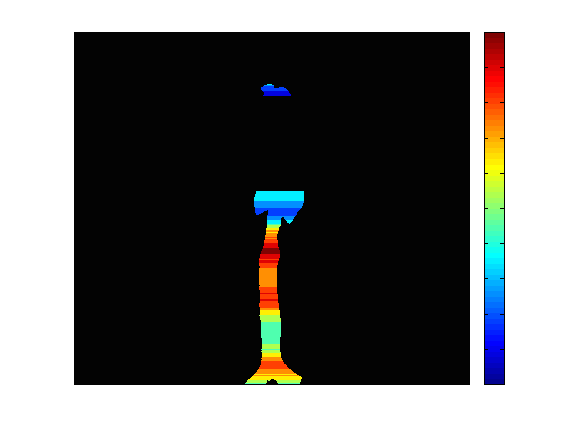
\includegraphics[width=\figwidth] {fig/CRL04_TracheaCarina_left.png}
    \end{tabular}
    \caption{ \label{fig:landmark_detection} Illustration of the likelihood of landmark TC. {\bf Left.} In most cases the detector located TC in a correct position. {\bf Right.} Even failure cases show the correct TC position as their second or third choice.
    }
  \end{center}
\end{figure}


% \begin{table}
%   \centering
%   \begin{tabular}{r || cccc}
%   & mean (mm) & std. (mm) & mean (px) & std. (px) \\
%   \hline
%   None & 4.7575 & 2.5314 & 18.6614 & 10.2052 \\
%   CHOG & 2.8812 & 1.6134 & 9.3357 & 6.6279 \\
%   \end{tabular}
%   \label{tab:landmarks}
%   \caption{Errors of landmark prediction methods of a 134 month subject (Fleck-005).
%    }
% \end{table}


Now let us apply the detector on dynamic data and see if it can handle landmark dynamics.
% I applied the detector on a 134 month old subject (Fleck-005).
Table~\ref{tab:Fleck_landmarks} summarized the landmark dynamics on TC, and my landmark detector using CHOG.
The landmark detector works well on the subjects Fleck 004 and Fleck 012.
But the detector perform bad on the other subjects.

\begin{table}
  \centering
  \begin{tabular}{|lcc|c|c|c|c|}
  \hline
  \multicolumn{3}{|c|}{Subjects} & \multicolumn{2}{|c|}{Landmark Dynamics} & \multicolumn{2}{|c|}{Landmark Prediction} \\
  \hline
  Id  & Age (m) & Weight (kg) & mean & std  & mean & std \\
  \hline
  Fleck 004 & 134.4   & 39.9  & 4.75 & 2.53 & 3.92 & 4.46 \\
  Fleck 007 & 114     & 25.2  & 4.21 & 6.16 & 7.58 & 5.92 \\
  Fleck 008 & 129.6   & 48.6  & 4.48 & 2.02 & 23.76 & 27.83 \\
  Fleck 009 & 130.8   & 37    & 1.85 & 1.35 & 30.32 & 3.16 \\
  Fleck 010 & 135.6   & 43.9  & 1.93 & 1.03 & 21.21 & 15.34 \\
  Fleck 012 &  42     & 14.5  & 1.48 & 1.03 & 1.47 & 0.69 \\
  Fleck 013 &  21.6   & 16.8  & 0.89 & 0.85 & 23.31 & 9.06 \\
  \hline
  \end{tabular}
  \caption{Qualitative measurement of the landmark detection. The prediction errors should be lower than the landmark dynamics. Currently, the detector only met this standard on the subjects Fleck 004 and Fleck 012.
   }
  \label{tab:Fleck_landmarks}
\end{table}
% My automatic landmark detector reduced the errors of the mean and standard deviation.
% However, the problem of outliers reminded for one frame.

% \begin{figure}[tb]
%   \begin{center}
%     \begin{tabular}{ccc}
%     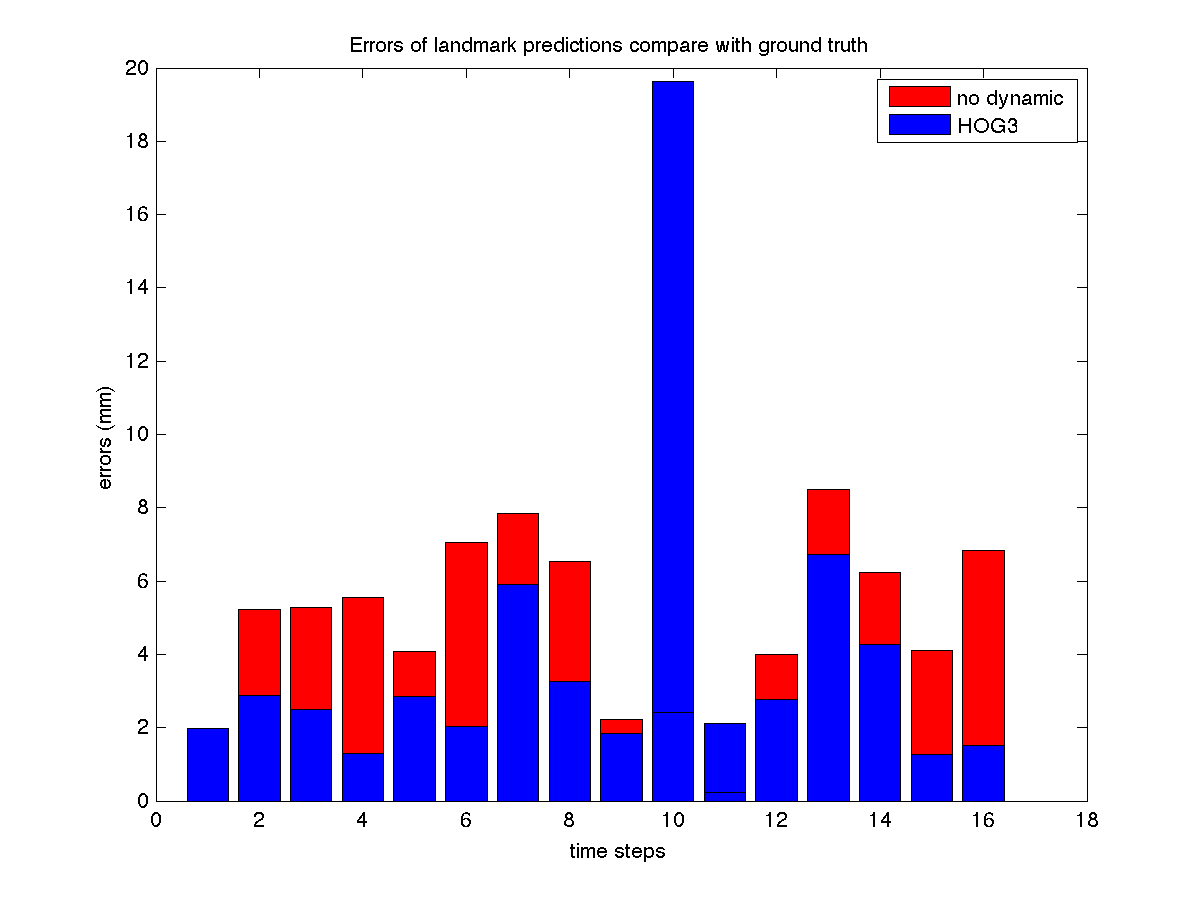
\includegraphics[width=0.4\linewidth] {fig/landmark_errors.png}
%     \end{tabular}
%     \caption{ \label{fig:landmark_errors} Illustration of the landmark prediction errors in each time step for subject Fleck-005. Red bar shows the errors of neglecting landmark dynamics and blue bar shows the errors from the proposed algorithm. Note that there is an outlier in time step 10.
%     }
%   \end{center}
% \end{figure}

\subsection{Dynamic airway analysis}
\label{sec:dynamic_airway_analysis}
\begin{figure}[tb]
  \begin{center}
    \begin{tabular}{ccc}
    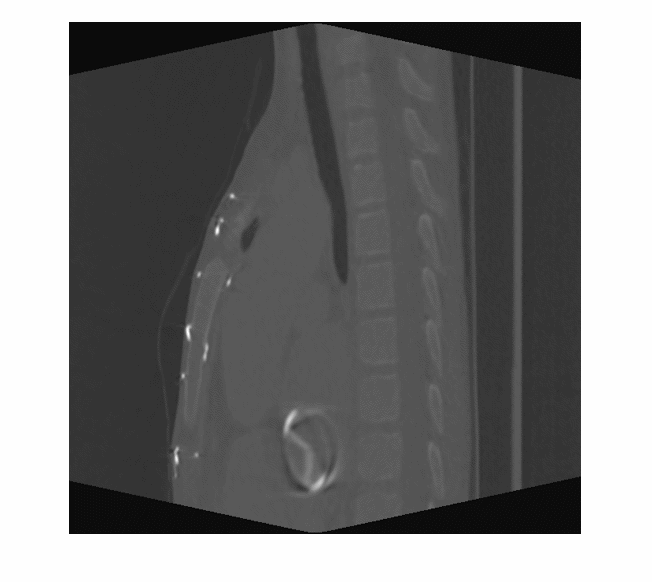
\includegraphics[height=\figheight] {fig/Fleck_007.png}
    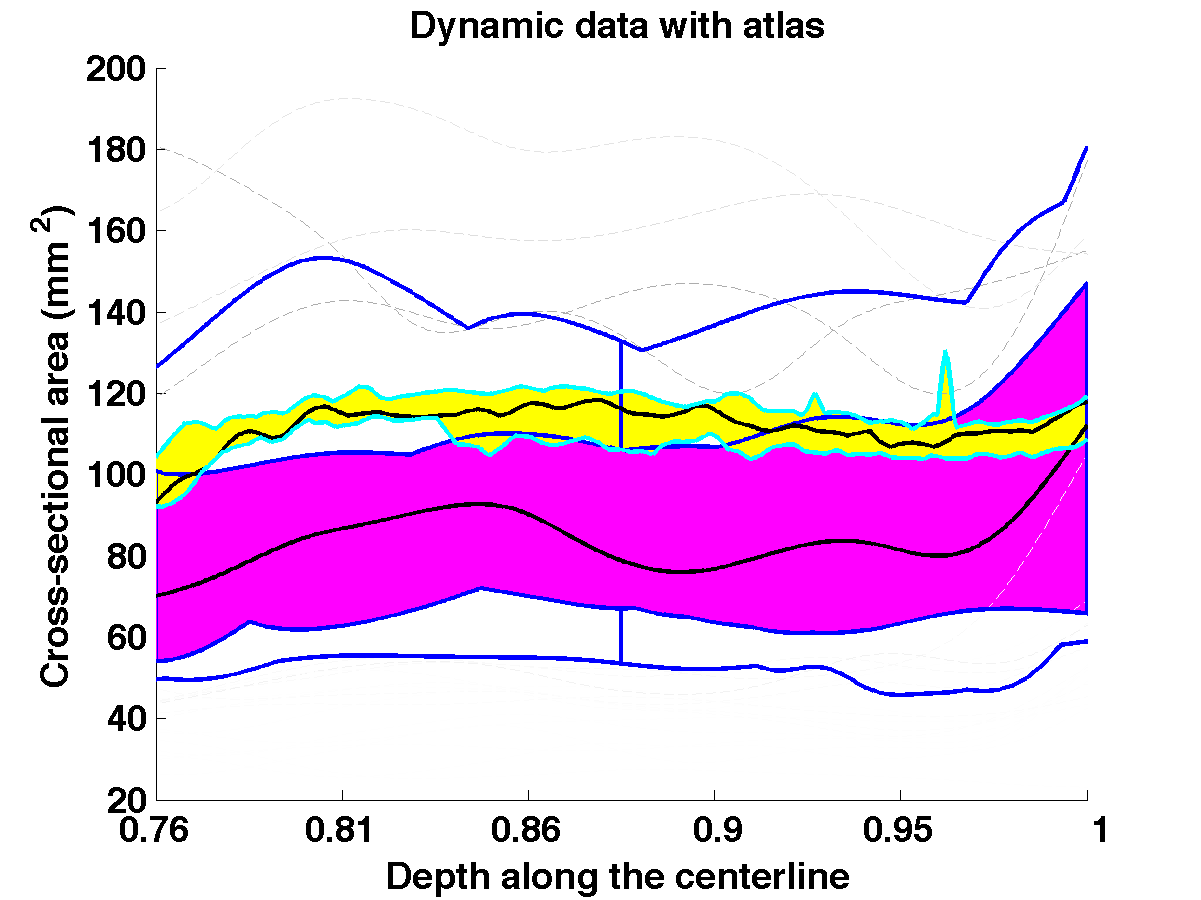
\includegraphics[width=\figwidth] {fig/Fleck_007_wfbplot.png} \\
    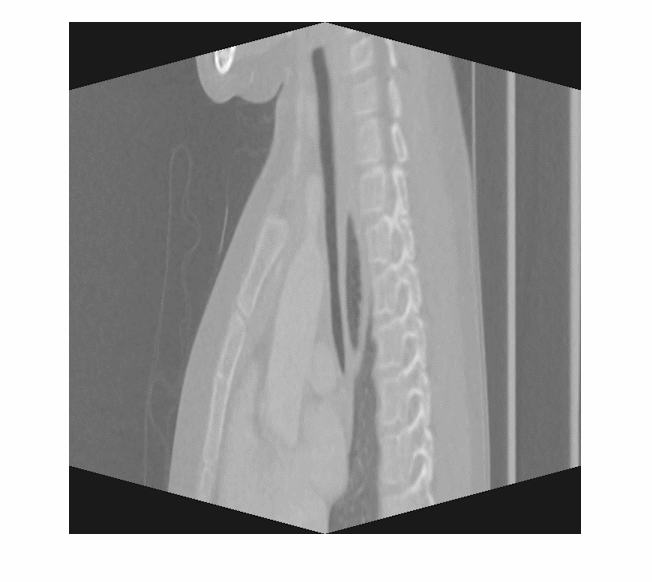
\includegraphics[height=\figheight] {fig/Fleck_008.png}
    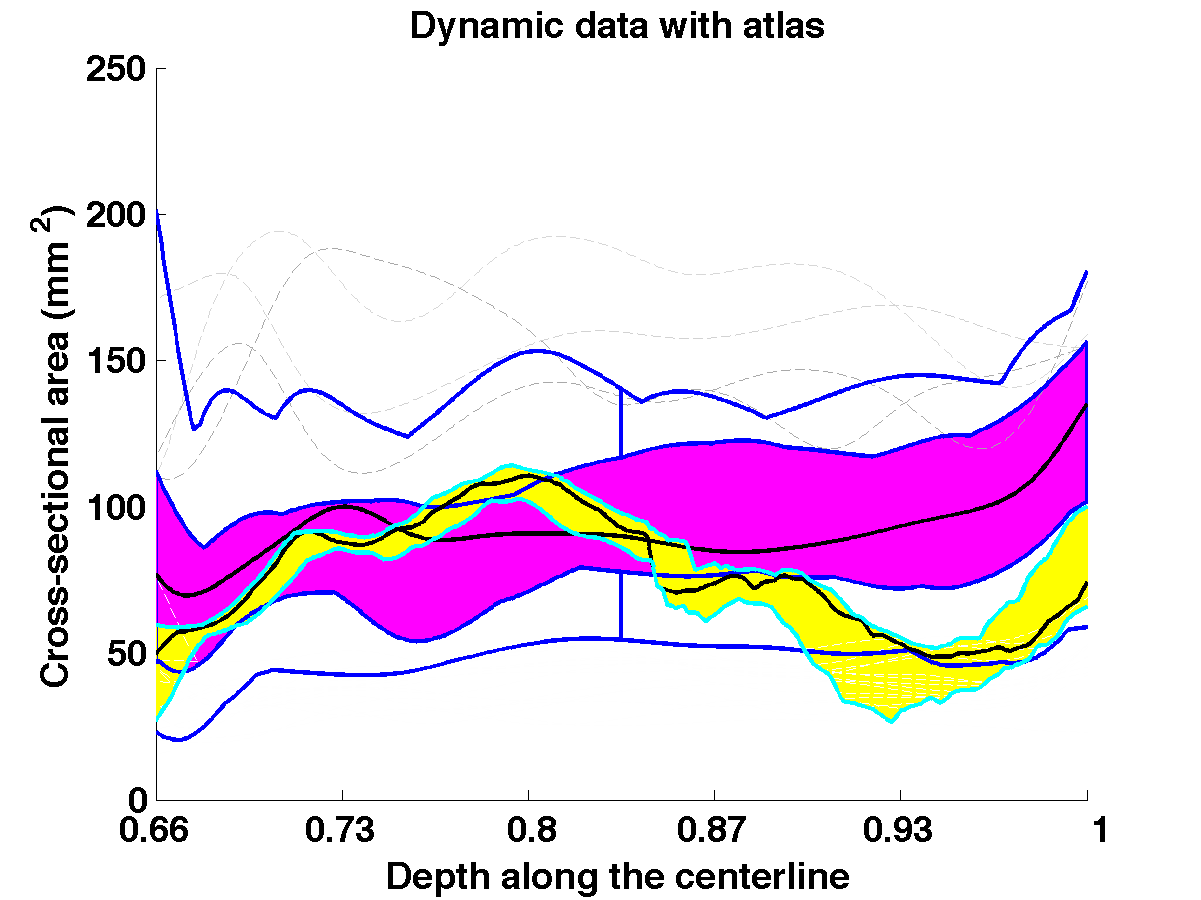
\includegraphics[width=\figwidth] {fig/Fleck_008_wfbplot.png} \\
    \end{tabular}
    \caption{ \label{fig:Fleck} Dynamic airway atlas for subject Fleck-007 and Fleck-008. {\bf Left.} A slice of dynamic data. {\bf Right.} The purple area is the interquartile range of the age-adapted normal control atlas. The blue curves are the maximum and the minimum of the normal control atlas. The yellow area is the entire estimation range of the dynamic subject over the different time steps. The depth is in a unified scale, where 0.66 is TVC and 1 is TC.
    }
  \end{center}
\end{figure}
I performed dynamic airway analysis using functional boxplots on real data provided by a physician.
The normal control atlas was built from 68 healthy subjects in control group using the method in~\cite{hong2014statistical}.
Figure~\ref{fig:Fleck} shows the qualitative results.
Here I compared these results with the comments from the doctor for two cases.

{\bf Fleck-007, 114 months.}
The subject seemed to have a narrow airway on the CT scan at the first glance.
However, comparing with the normal control atlas, this subject definitely had an airway size larger than average normal control data.
Also, the doctor's comment was ``No significant change in the trachea or bronchi during cough maneuver. No evidence of tracheobronchomalacia.'', which qualitatively agrees with the analysis result.

{\bf Fleck-008, 129.6 months.}
For this subject the airway seemed normal in one slice.
Yet it was considered narrowed compared with the normal control atlas, and it had large dynamics especially from the depth 0.87 to 1.
The depth 0.66 means TVC and 1 means TC.
So the subject had narrowed trachea near TC.
Quote the doctor's comment ``Dynamic, 2.5 cm long narrowing of the mid to distal thoracic trachea caused by the adjacent left-sided aortic arch. The luminal diameter of the trachea changes from 11 mm during diastole to 5 mm in systole'', the subject did show problems in the mid to distal thoracic trachea, the analysis results qualitatively agree with the observation.

Table~\ref{tab:Fleck} shows qualitative experiments on our dataset.
I measured the cross-sectional area changes during the breathing.
Studies suggested a subject with over 50\% changes of cross-sectional area during the breathing might be a suspected tracheomalacia~\cite{chung2011ct, boiselle2009tracheal, hasegawa2003tracheomalacia}. 
Our system computed collapsed dynamics from 4D CT images, and gave qualitative measurement that agree with the studies and the diagnosis from our collaborator.
\begin{table}
  \centering
  \begin{tabular}{|lcc|c|c|c|c|c|c|c|}
  \hline
  \multicolumn{3}{|c|}{Subjects} & \multicolumn{3}{|c|}{Dynamics} & \multicolumn{3}{|c|}{Collapsed Dynamics} & Diagnosis \\
  \hline
  Id  & Age (m) & Weight (kg) & min & mean & max  & min & mean & max &\\
  \hline
  Fleck 004 & 134.4  & 39.9   & 4\% & 14\% & 82\% & 12\%& 22\%& 82\% & Normal \\
  Fleck 007 & 114 & 25.2      & 4\% & 8\%  & 20\% & 0\% & 0\% & 0\% &  Normal \\
  Fleck 008 & 129.6   & 48.6  & 5\% & 22\% & 54\% & 31\%&39\% &53\% & Tracheomalacia \\
  Fleck 009 & 130.8   & 37    & 7\% & 15\% & 43\% & 0\% & 0\% & 0\% &Normal \\
  Fleck 010 & 135.6   & 43.9  & 4\% & 12\% & 19\% & 0\% & 0\% & 0\% & Normal \\
  % Fleck 011 &  51.6   & 16.6        &&&     &      &     && Tracheomalacia \\
  Fleck 012 &  42     & 14.5  & 11\% & 18\% & 44\% & 0\% & 0\% & 0\% &Normal \\
  Fleck 013 &  21.6   & 16.8  & 1\% & 20\% & 68\% & 34\% & 56\% & 68\% & Tracheomalacia \\
  % Fleck 014 &   7.2   &  6.5        &&&     &      &     && Tracheomalacia \\
  \hline
  \end{tabular}
  \caption{Qualitative measurement of atypicality of dynamic subjects. The column Dynamics measures the entire dynamics through the airway. The Collapsed Dynamics measures only on the region which cross-sectional area is smaller than the normal control atlas.
  Diagnosis is judged by our physician collaborator.
   }
  \label{tab:Fleck}
\end{table}




% \begin{table}
%   \centering
%    \caption{Errors of landmark prediction methods of a 134 month subject (Fleck-005).
%    }
%   \begin{tabular}{l | rrrr}
%   Subjects & Ages (m) & Weight (kg) & \multicolumn{3}{c} Dynamics (entire) & Dynamics (focus) \\
%   \hline
%   Fleck 007 (11) & 114   & 25.2 \multicolumn{3} && \\
%   Fleck 008 (16) & 129.6 & 48.6 && \\
%   Fleck 009 (8) & 130.8 & 37 && \\
%   Fleck 010 (16) & 135.6 & 43.9 && \\
%   Fleck 011 (11) & 51.6 & 16.6 && \\
%   Fleck 012 (8) & 42 & 14.5 && \\
%   Fleck 013 (8) & 21.6 & 16.8 && \\
%   Fleck 014 (8) & 7.2 & 6.5 && \\
%   \end{tabular}
%   \label{tab:Fleck}
% \end{table}

\section{Discussion}
\label{sec:discussion}
This work proposed an automatic framework for processing a 4D CT image of pediatric airway and providing informative visualization for further analysis.
The current approach of data registration using detected landmarks has two issues.
First, the detection has outliers.
The outliers could be eliminated by examination the distance of each detected result between the detection mean.
Yet more powerful features might need to be developed.
Second, finding correspondents between a subject without enough landmarks to its statical atlas is handled by heuristics.
To fully solving this problem, reducing the rely on landmarks is necessary.
Since the within subject deformations were not dramatic, as Guerrero et al.'s suggestion in~\cite{guerrero2006dynamic}, a deformable image based registration within a subject would be a proper next step.

While the results has showed dynamic ranges and a comparison between dynamic data to normal control atlas, a more straightforward metric which quantifies atypicality of subjects would be very appreciated.
A reasonable next approach would be designed a metrics to evaluate the dynamics of airway.
A long term goal of this project is to develop a theory of 4D CT atlas building of pediatric airways and aim for going beyond to other parts of human body.

\bibliographystyle{splncs}
\bibliography{prp}

\end{document}
